\section{Modèle 3D}
Si l'on veut permettre à l'utilisateur de se repérer dans le bâtiment, il faut commencer par modéliser ledit bâtiment. Un projet d'étudiant a, dans le passé, permis de générer une première version d'une modélisation, à l'aide du logiciel \emph{Blender} \cite{blender-website}. Cependant, après l'avoir inspectée, il s'est avéré qu'elle comportait beaucoup de polygones inutiles, voir Figure \ref{fig:model-toomanypolygons}.

\begin{figure}[h!]
	\centering
	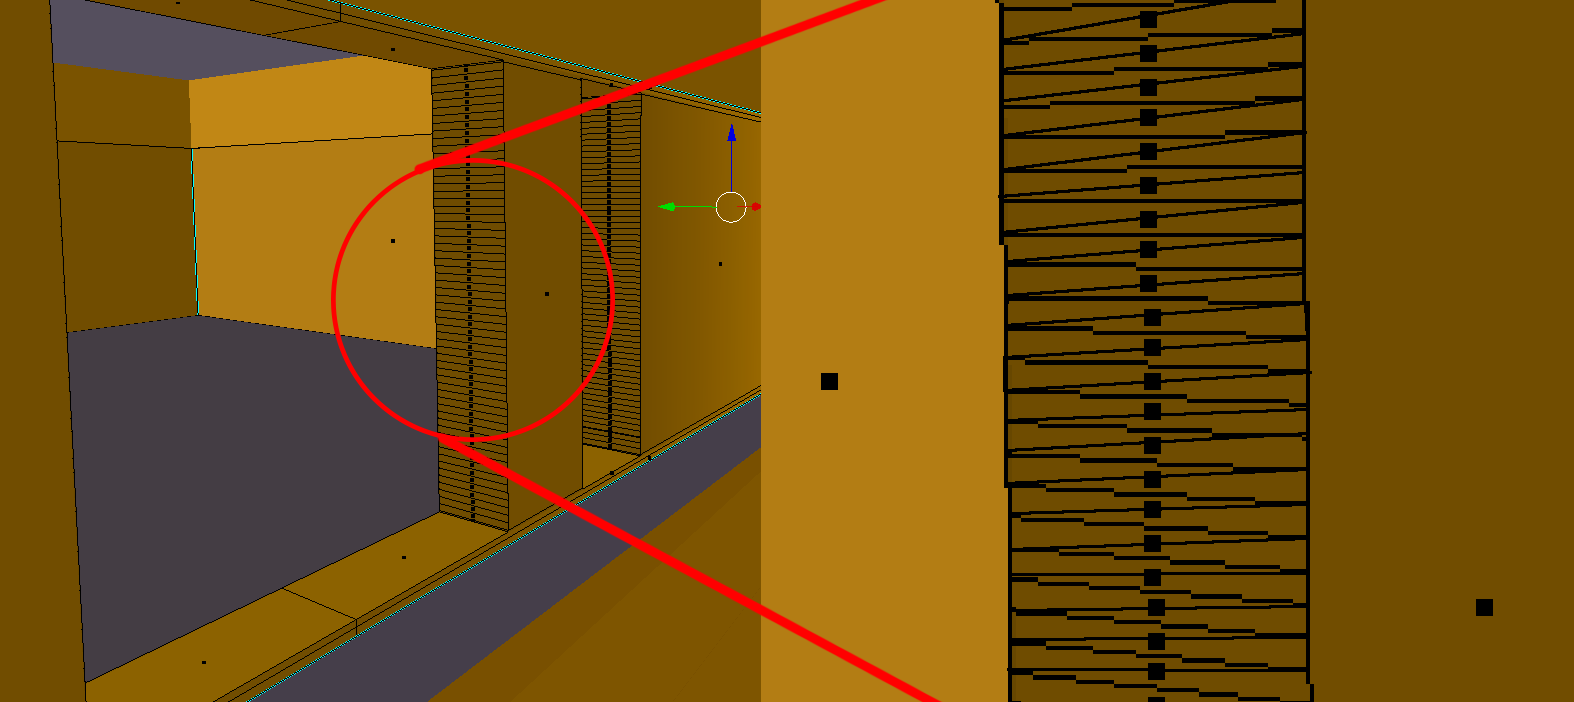
\includegraphics[width=0.9\linewidth]{model-TooManyPolygons}
	\caption{Un exemple des défauts du modèle}
	\label{fig:model-toomanypolygons}
\end{figure}

A ce problème existent deux solutions: soit effectuer un \textit{geometry clean up}, qui consiste à supprimer le surplus de polygones, soit modéliser à nouveau le bâtiment. Sachant que je ne possède aucune connaissance en modélisation, il a été jugé plus adéquat de modéliser une nouvelle fois l'école, ceci dans un but d'apprentissage plus logique si l'on commence par les bases.

L'environnement de modélisation choisi est \emph{Autodesk 3ds Max} \cite{autodesk-3dsmax}. Ce logiciel professionnel offre beaucoup plus de fonctionnalités que Blender ainsi qu'une licence étudiant gratuite, ce qui en fait une bonne solution pour la modélisation.


\subsection{Modélisation géométrique}
Pour modéliser correctement l'école, il est important de se munir des plans du bâtiment, car effectuer toutes les mesures sur place et à main levée est source d'erreurs et de pertes de temps. Les seuls plans qu'il a été possible de récupérer sont les plans de sols, les hauteurs ont donc été calculées par ratio. Ici, le but n'est pas la précision exacte du modèle mais de réaliser où l'on se trouve. Ce n'est donc pas un problème d'avoir un quelconque manque de précision sur les hauteurs des étages.

D'abord, la forme des murs a été reportée depuis le plan (Figure \ref{fig:model-formemur}) sur \textit{Autodesk 3ds Max} (Figure \ref{fig:model-formemurautodesk}). Ensuite, la forme des murs a pu être extrudée afin d'obtenir des objets 3D, voir Figure \ref{fig:model-murextrude}. A partir de ce modèle, il a été possible de commencer à pouvoir travailler la véritable forme du bâtiment, c'est-à-dire de modéliser les pas de portes et fenêtres, les sols et plafonds, ainsi que les cages d'escaliers (Figure \ref{fig:model-onefloor} et \ref{fig:model-onestairs}), pour obtenir, au final, un modèle complet du Campus Arc 2 de la Haute-Ecole Arc de Neuchâtel (Figure \ref{fig:model-all}).

\begin{figure}
\centering
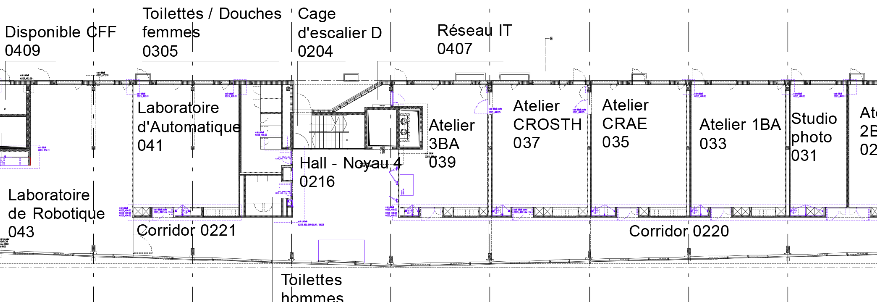
\includegraphics[width=0.9\linewidth]{model-FormeMur}
\caption{Plans du bâtiment utilisés pour la modélisation.}
\label{fig:model-formemur}
\end{figure}

\begin{figure}
\centering
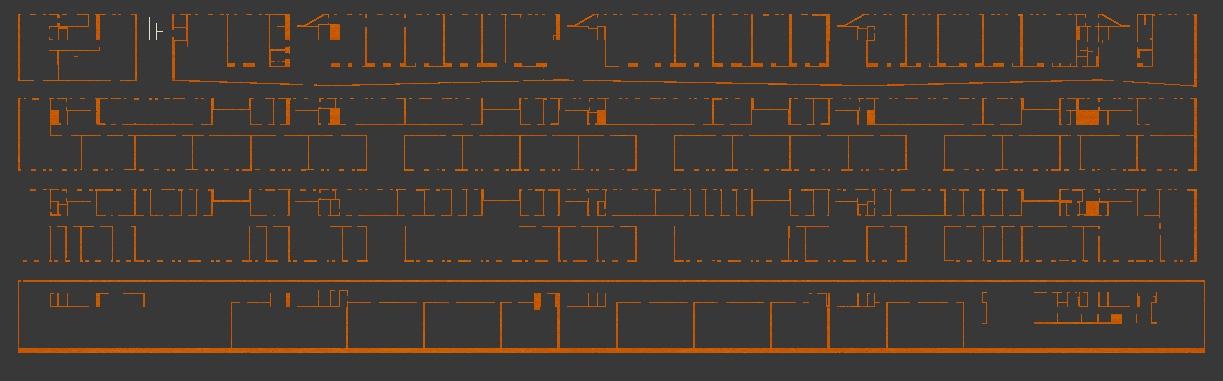
\includegraphics[width=0.9\linewidth]{model-FormeMurAutodesk}
\caption{Le résultat après le report du plan sur \textit{Autodesk 3ds Max}.}
\label{fig:model-formemurautodesk}
\end{figure}

\begin{figure}
	\centering
	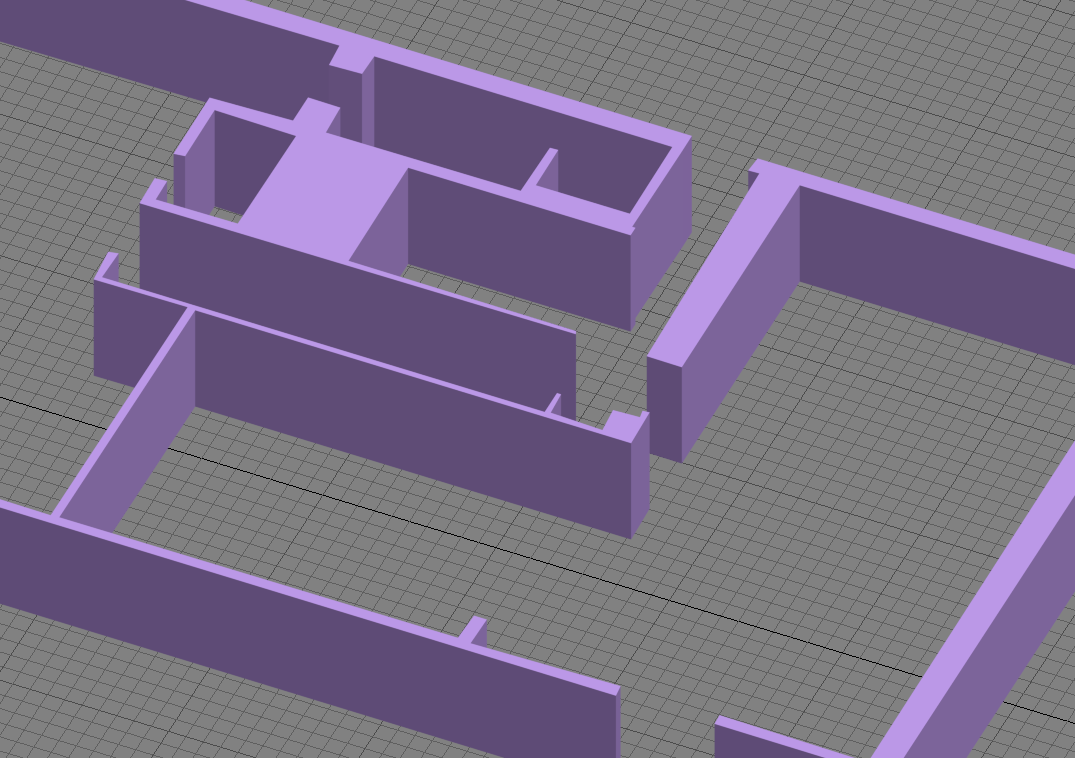
\includegraphics[width=0.9\linewidth]{model-MurExtrude}
	\caption{Les murs du bâtiment après extrusion.}
	\label{fig:model-murextrude}
\end{figure}

\begin{figure}
	\centering
	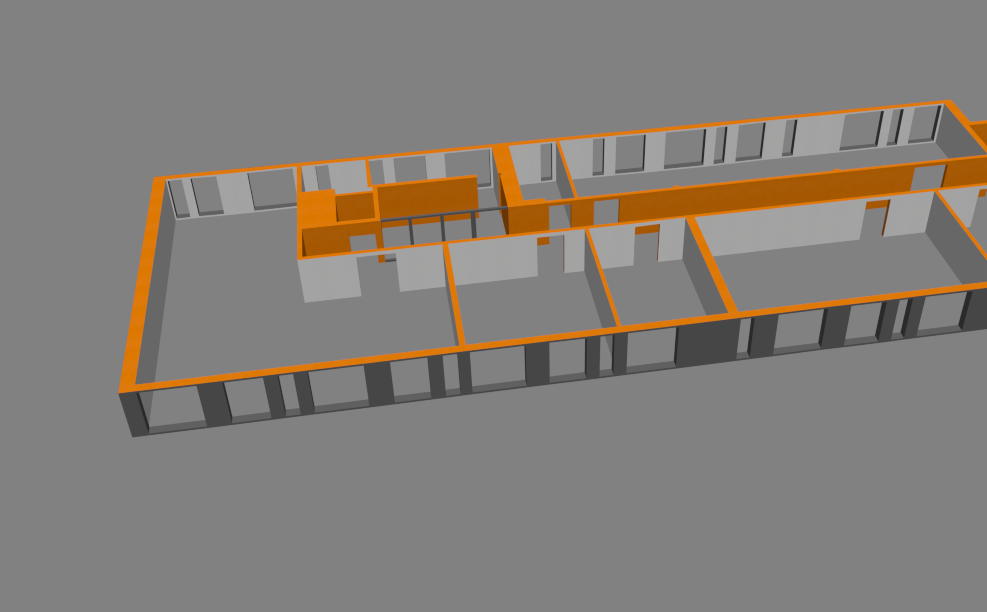
\includegraphics[width=0.9\linewidth]{model-OneFloor}
	\caption{Un étage du bâtiment.}
	\label{fig:model-onefloor}
\end{figure}

\begin{figure}
	\centering
	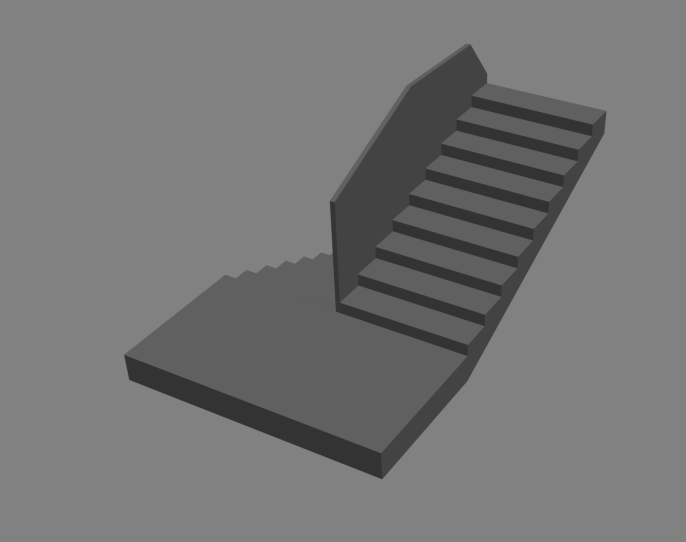
\includegraphics[width=0.9\linewidth]{model-OneStairs}
	\caption{Un exemple d'escalier}
	\label{fig:model-onestairs}
\end{figure}

\begin{figure}
	\centering
	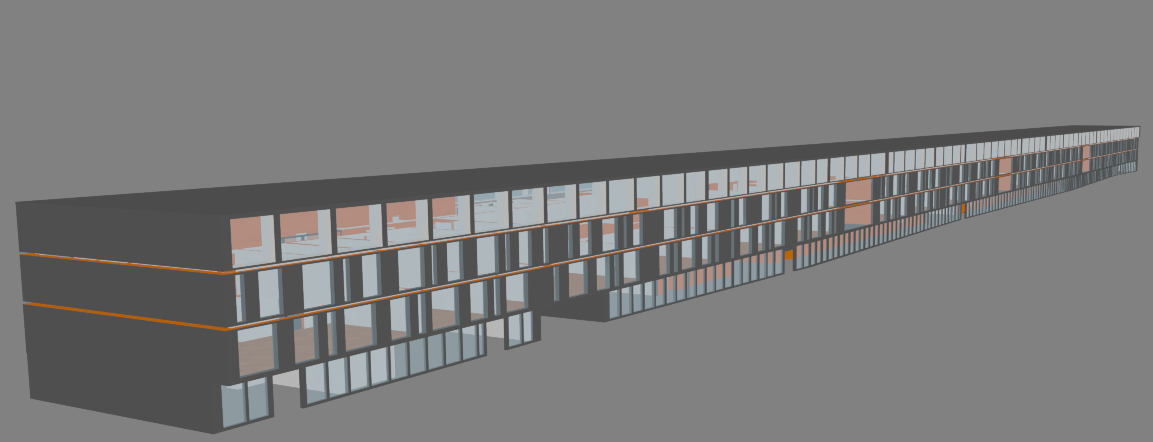
\includegraphics[width=0.9\linewidth]{model-All}
	\caption{Le modèle du bâtiment complet.}
	\label{fig:model-all}
\end{figure}


\subsection{Texturisation du modèle}
Maintenant que nous avons un modèle du bâtiment, nous voulons que les utilisateurs le reconnaissent. L'étape de texturisation doit servir à cela. On va appliquer des textures qui correspondent aux véritables matériaux afin de faire ressembler le modèle au maximum à la réalité.

\subsection{Exportation et importation}
Afin de pouvoir utiliser notre modèle avec threejs, il faut employer un format de fichier pour pouvoir le transférer. Plusieurs formats ont étés analysés et expérimentés. Il en ressort que celui qui est le mieux supporté par threejs est le format \emph{JSON}\cite{wiki-json}. Il est pourtant simple d'exporter depuis \textit{Autodesk 3ds Max} en format \emph{OBJ}, mais threejs supporte mal le grand nombre de polygones avec ce format (voir Figure \ref{fig:import-objfail}).

\begin{figure}
	\centering
	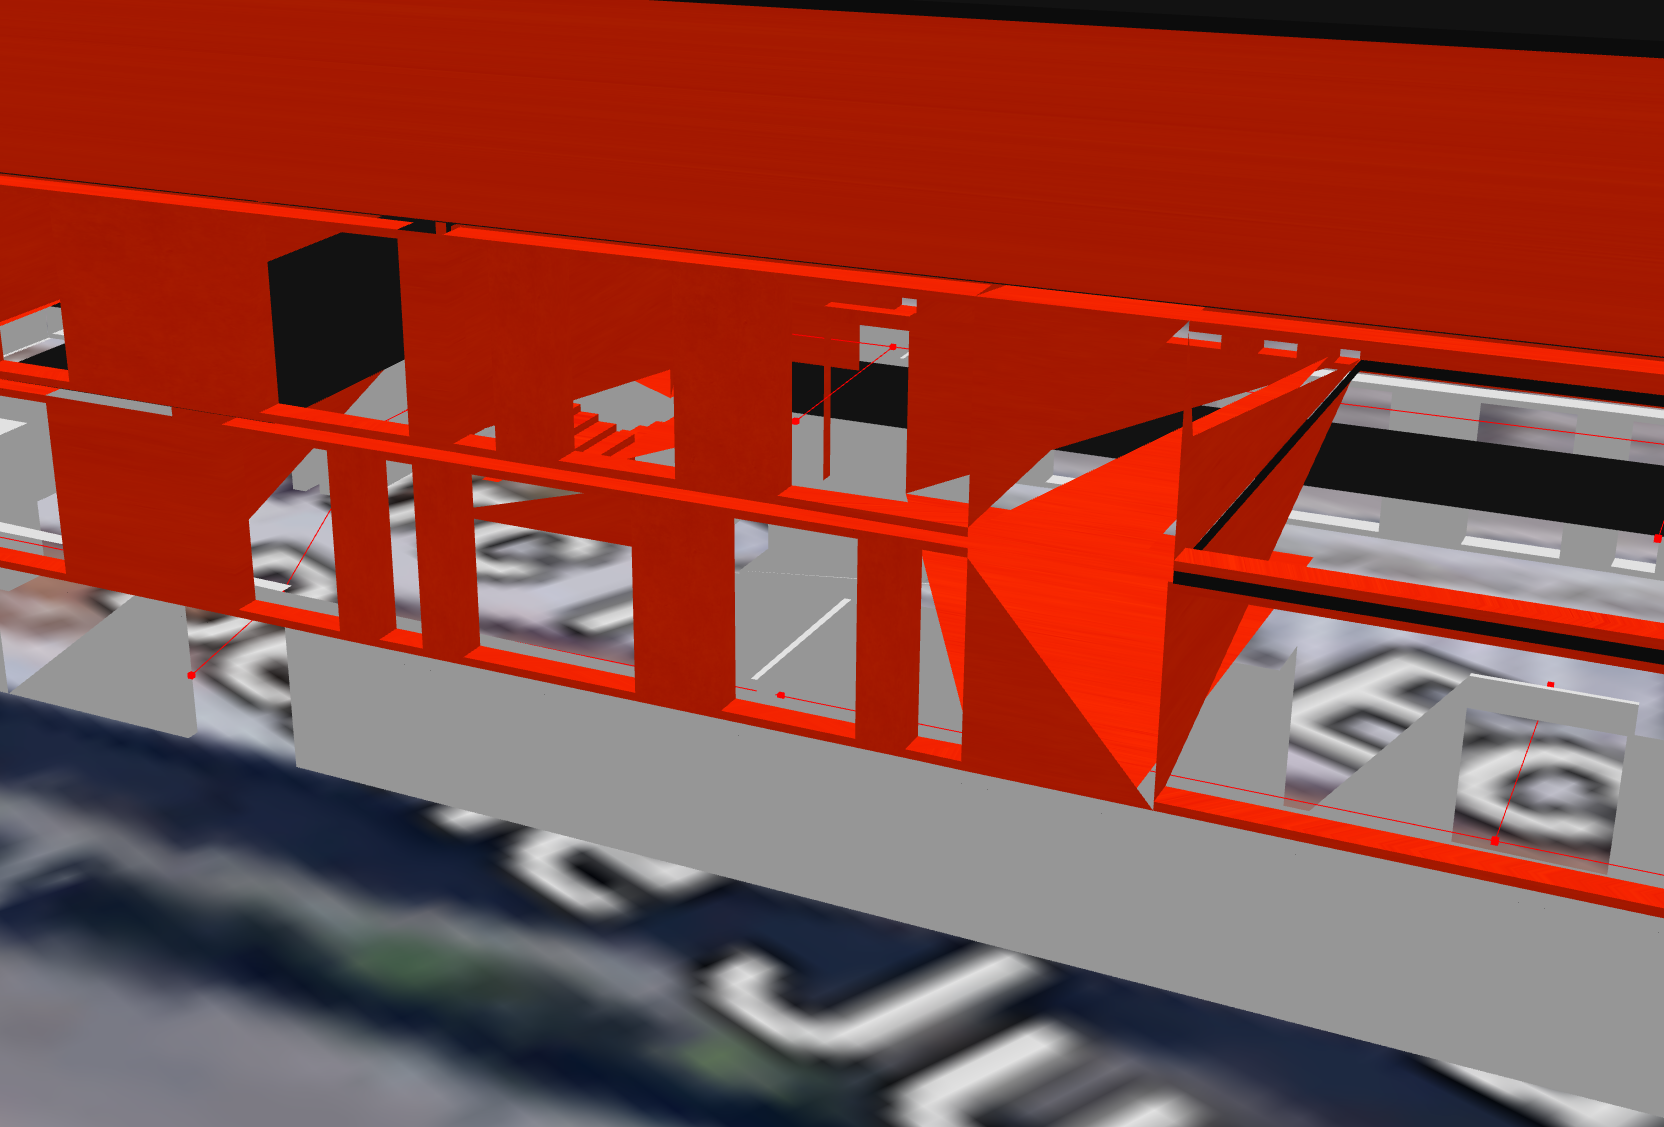
\includegraphics[width=0.9\linewidth]{import-ObjFail}
	\caption{threejs supporte mal les modèles composés de beaucoup de polygones en format OBJ.}
	\label{fig:import-objfail}
\end{figure}

\textit{Autodesk 3ds Max} ne permet pas, par défaut, d'exporter un modèle en format JSON. Il est néanmoins doté d'un système de plugins qu'il est possible de créer et d'ajouter au logiciel. Les développeurs de \textit{threejs} l'ont déjà pensé et mettent à disposition un plugin permettant d'exporter notre modèle au format JSON. Cependant, la librairie étant encore en alpha, tout n'est pas toujours à jour, il a donc fallu modifier le code (écrit en Maxscript \cite{autodesk-maxscript}) afin qu'il corresponde aux derniers standards de la librairie et que l'on puisse l'utiliser sans problème. Du côté WebGL, la librairie offre des utilitaires permettant de charger ces fichiers facilement.